\section{Confirmation: useful succession, held product admission}
\label{sec:results}

The single frozen campaign ran from 01:10:38 to 01:15:28 UTC on 25 October 2026, taking 289.289\,s wall time.
Measured campaign CPU was 171.115\,s in Python and 123.638\,s in its workbench children. All 168 registered trials
completed without a source change, manual phase trigger, trial failure or declared resource violation. The
post-run freeze check reverified all 32 files. No additional confirmatory campaign was started.

\subsection{Complete service coverage, without an expanded envelope}

Every treatment qualified 492 of 492 offered useful outputs. Across the campaign, 3,444 useful outputs and
42 maintenance outputs passed the independent numerical checker. All 168 unsupported negative-conductance
requests were explicitly refused. Because the competent controls achieved the same coverage, this result
shows reliable implementation in the declared envelope; it does not show a newly feasible mission set.

\begin{table}[htbp]\centering\small
\begin{tabularx}{\linewidth}{@{}Yrrrr@{}}\toprule
Treatment & Qualified & Mean CPU (s) & Successors & Fresh child uses \\\midrule
Flywheel & 492/492 & 1.731 & 18 & 156 \\
Conventional reuse & 492/492 & 1.745 & 18 & 156 \\
Direct warm CG & 492/492 & 1.764 & 0 & 0 \\
Parent rebuilt & 492/492 & 1.752 & 24 & 228 \\
Independent equivalent & 492/492 & 1.759 & 24 & 228 \\
Native refactor + cache & 492/492 & 1.742 & 0 & 0 \\
No reinvestment & 492/492 & 1.759 & 0 & 0 \\\bottomrule
\end{tabularx}
\caption{Whole-participant CPU per independent stream. ``Successors'' denotes low-rank instruments; the native
refactor arms create ordinary current-operator factors. The two forced construction ablations are diagnostic,
so their 24 children are not 24 economic promotions. All treatments can retain legitimate ordinary state.}
\label{tab:main}
\end{table}

\begin{figure}[htbp]\centering
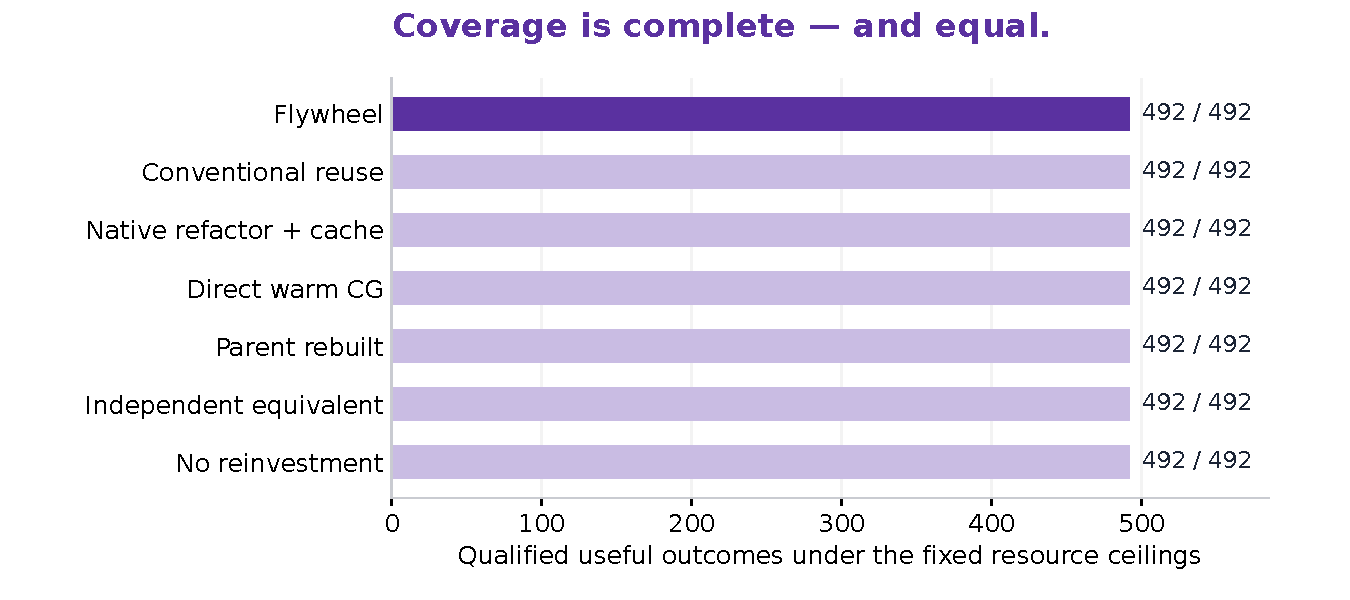
\includegraphics[width=\linewidth]{figures/qualified-coverage.pdf}
\caption{The same qualified coverage under the fixed resource ceilings. Useful computation is real, but more
inherited assets do not expand the tested mission envelope beyond competent conventional execution.}
\end{figure}

\subsection{The primary gate fails}

The flywheel's mean whole-participant CPU is 1,730.732\,ms, compared with 1,742.402\,ms for native refactorization
and caching. The ratio is $R=0.9933025$, with registered paired, stratified bootstrap interval
$[0.9668841,1.0264574]$. The point estimate is 0.67\% lower; the interval spans both benefit and loss and does not
support the required 5\% improvement. \textbf{Product admission is HOLD.}

Against equally enabled conventional reuse, the ratio is $0.9915906$ with interval $[0.9639719,1.0191137]$.
This passes the prespecified 10\% noninferiority guard. The conventional policy has the same capability choices;
its agreement with the flywheel is expected evidence of enabled conventional reuse, not evidence of unique AGI
superiority. The direct-specialist contrast is also inconclusive end to end: ratio $0.9812102$, descriptive
interval $[0.9437037,1.0200646]$.

\begin{figure}[htbp]\centering
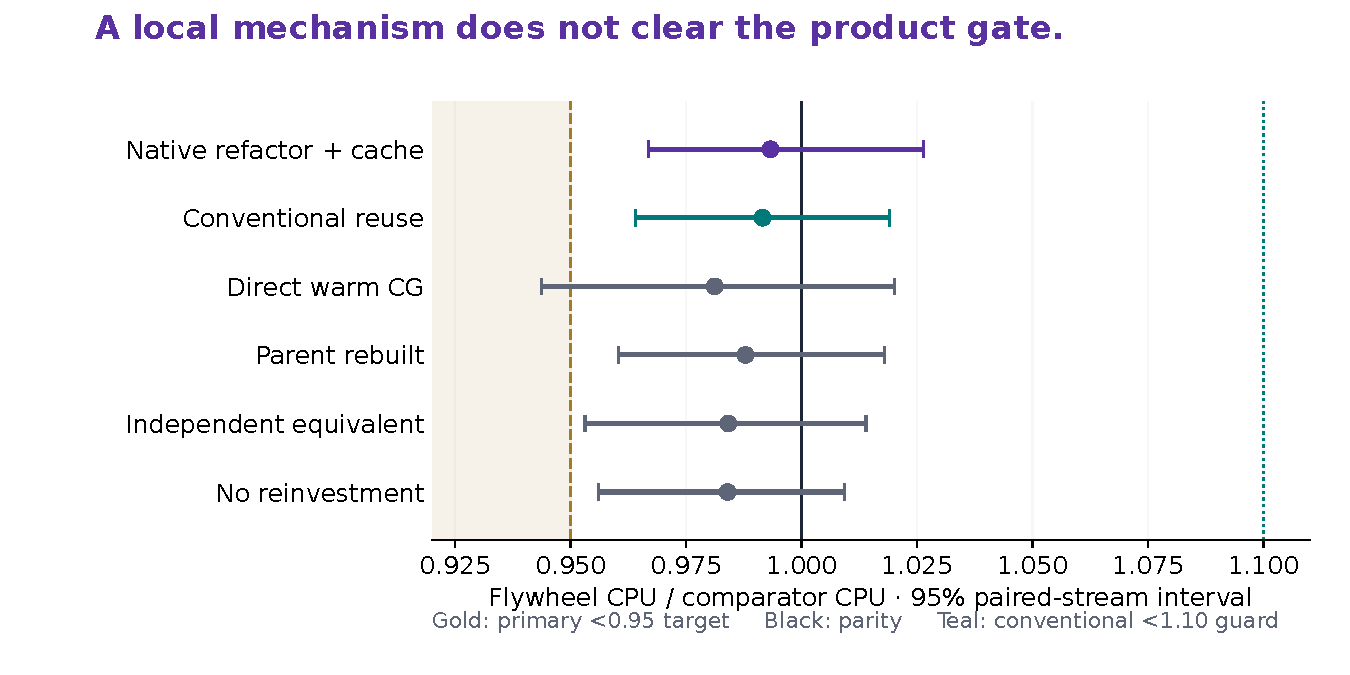
\includegraphics[width=\linewidth]{figures/full-cost-comparison.pdf}
\caption{Ratios of mean whole-participant CPU, with paired-stream percentile intervals. The primary native-refactor
interval does not clear the registered 0.95 threshold. Other contrasts are descriptive; conventional reuse also
has a separately registered 1.10 noninferiority guard. Lower ratios favor the flywheel.}
\label{fig:cost}
\end{figure}

\subsection{A real successor: what transfers and what it costs}

In the eighteen eligible low-rank flywheel streams, C makes one batched parent call to compute the two-column
response basis, followed by a second parent call while qualifying the changed-network response. Later fresh D
requests make 156 additional parent calls and all qualify. The independent audit ties the selected edges to
actual accepted B08 flows and finds no paired input divergence across treatments. This closes the earlier
edition's gap between a stored parent pointer and a fresh qualified output that actually uses its parent.

The first registered stream, seed 684407853, is a concrete example rather than a selected best case. A solves
2,304 nodes and 4,512 edges, with relative residual $2.44\times10^{-15}$. The retained parent identity begins
\artifact{88d25bbb31dd}. B08 has a new load and a different checked response. Its two highest-flow edges, indices
2991 and 3320, receive the prescribed positive increments. C constructs child \artifact{19ec0f844656}, binding
B08 receipt \artifact{f492b0100a47}; its persisted update arrays occupy 77,408 bytes. Fresh D01 uses both that child
and its parent, with relative residual $1.52\times10^{-15}$. The subsequent grounding change refuses old scope
and uses the specialist; negative conductance is refused without a result.

\begin{figure}[htbp]\centering
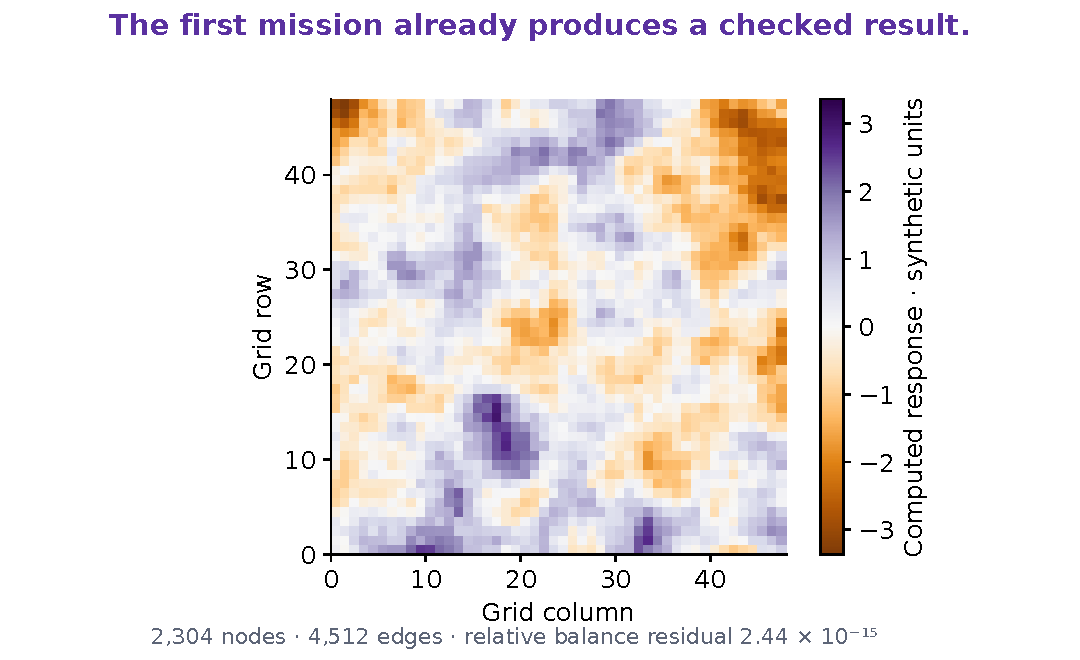
\includegraphics[width=.85\linewidth]{figures/first-useful-result.pdf}
\caption{A useful result before any succession claim: the first registered stream's independently checked node
response. The full inputs and output vector are preserved. Colors represent this synthetic numerical solution,
not an observed physical network.}
\end{figure}

A clean construction intervention compares the same low-rank constructor with and without a retained factor.
In the recurring regime, C's measured algorithm phase averages 1.61\,ms with inheritance and 7.88\,ms with
native reconstruction; the equivalent-parent version averages 6.43\,ms. The phase includes construction,
one qualification solve and persistence. It is not a pure factorization benchmark. The end-to-end C action
averages 51.57, 54.27 and 58.12\,ms respectively, showing how much overhead can dilute that local difference.

Native C averages 10.21\,ms in its algorithm phase and 66.53\,ms for its action in that regime. However, its
code path performs an additional full input-scope scan that the parent-based constructor replaces with bounded
parent/update checks; both receive the same final checker. Therefore this secondary gap mixes construction
and validation work. It must not be advertised as an isolated algebraic speedup against an equally optimized
native constructor. The primary whole-workflow result already remains held.

\subsection{Maintenance and the simpler alternative}

The flywheel retains the native alternative in all six wide-change streams rather than building the proposed
low-rank instrument. In the maintenance regime, its mean full cost is 2,569.456\,ms, above native refactorization's
2,538.358\,ms and direct CG's 2,470.167\,ms. Portable factor validation and restoration are substantive work:
flywheel restore actions average 152.02\,ms, while direct CG's matched recovery action averages 81.29\,ms.
In the rare regime, flywheel CPU is also slightly above native refactorization, 1,088.842 versus 1,086.199\,ms.
These are descriptive regime findings with six streams each, not independently significant subgroup claims.

\begin{figure}[htbp]\centering
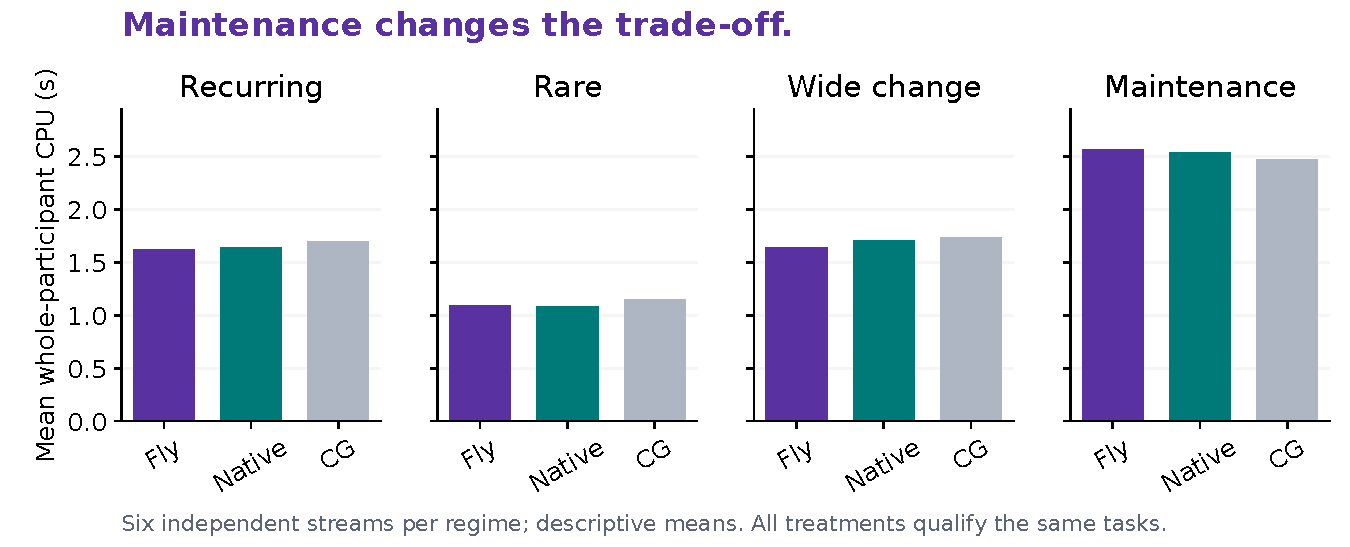
\includegraphics[width=\linewidth]{figures/regime-costs.pdf}
\caption{When reuse helps locally and when its complete burden remains uncompetitive. Every regime has equal
qualified coverage. Maintenance can make a simpler solver preferable even when the inherited instrument is correct.}
\end{figure}

Only 3.274\,s of the flywheel's 41.538\,s total participant CPU lies in the recorded algorithm phases; these
phases themselves include preflight and persistence work. The independent checker consumes 4.860\,s,
workbench child CPU 15.579\,s, and shared setup/custody/aggregate-artifact work 7.129\,s. Other Python binding,
serialization and transport work fills the remaining difference. These are disjoint components only after
subtracting the nested measurements correctly; action CPU must not be added again to its constituent costs.
A faster solve does not automatically make the complete service proportionally faster.

\subsection{Resource feedback is executed, not self-financing growth}

Across 24 flywheel streams, accepted B work transfers 9,600\,ms of unused service quota to the released-capacity
account. The eighteen successor actions debit 1,034.057\,ms of actual dispatched CPU. Construction is therefore
funded within the reassigned allowance and does not borrow the separate research account. The native and direct
controls receive the same release opportunity; an abundance of unused reservation is not an inherited advantage.

These transfers originate in externally supplied capacity. The paired comparison does not establish the
required incremental productivity gain, and a 1,034.057\,ms child debit cannot be relabelled profit or recovered
research investment. The remaining released allowance is unused endowment. No monetary margin, customer demand,
paid adoption or increasing improvement rate was measured.

\subsection{Independent verification and its limits}

The frozen second implementation audits 168 trials, 3,654 raw records, 3,486 accepted numerical outputs and
5,334 artifact identities with zero reported issues and zero paired-input divergences. It reproduces the exact
primary point ratio. Its independently arranged bootstrap draws give interval $[0.9672105,1.0271364]$; the small
endpoint difference is Monte Carlo/resampling-layout variation, not another experiment. Both frozen analyses
leave product admission on HOLD. Its conventional interval $[0.9650167,1.0194604]$ also passes the registered guard.

The checker and aggregator are separately implemented, but their reviewer belongs to the same commissioned team
and helped correct executor validation before the freeze. CPU observations cannot be reconstructed from hardware
after the fact; the audit reconciles their stored accounting boundaries. Parent calls are producer instrumentation,
independently attributed to output and lineage records, not an external instruction trace. These limits are part
of the evidence, not grounds for upgrading institutional authority.
